\setAuthor{Joonas Kalda}
\setRound{lahtine}
\setYear{2022}
\setNumber{G 2}
\setDifficulty{2}
\setTopic{TODO}

\prob{Pliiats}
\begin{wrapfigure}{r}{0.1\textwidth}
\raisebox{3pt}[\dimexpr\height-0.6\baselineskip\relax]{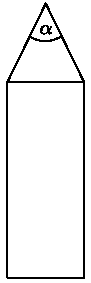
\includegraphics[scale=0.95]{2022-lahg-02-yl.pdf}}
\vspace{-55pt}
\end{wrapfigure}
Pliiatsi kahe näpu vahel õhus hoidmiseks tuleb rakendada sama jõudu olenemata sellest, kas hoitakse kinni tipust või külje pealt. Näpu hõõrdetegurid pliiatsi küljega ja teritatud osaga on vastavalt $\mu_1 = \SI{0,3}{}$ ja $\mu_2 = \SI{0,5}{}$. Milline on pliiatsi tipunurk $\alpha$?



\hint

\solu
Et kehtiks horisontaalne jõudude tasakaal, peavad pliiatsi hoidmisel mõlemad sõrmed rakendama sama jõudu. Olgu pliiatsi mass $m$ ja pliiatsi hoidmiseks vajalik jõud ühelt sõrmelt $N$. Pannes kirja vertikaalsuunalised jõudude tasakaalud mõlema hoidmisasendi jaoks, saame võrrandid,
\[2\mu_1 N = mg ,\]
\[2 \cos\frac{\alpha}{2}\mu_2N= 2\sin\frac{\alpha}{2}N + mg .\]
Lahendame süsteemi,
\[\sin\frac{\alpha}{2} N + \mu_1 N = \cos\frac{\alpha}{2}\mu_2 N .\]
Teeme asenduse $\sin{\frac{\alpha}{2}} = x$,
\[x + \mu_1 = \mu_2 \sqrt{1-x^2},\]
\[(x + \mu_1)^2 = \mu_2^2(1-x^2),\]
\[(1+\mu_2^2) x^2 + 2\mu_1 x + (\mu_1^2 - \mu_2^2) = 0.\]
Ruutvõrrandi lahenditeks on $x_1 \approx 0.191$ ja $x_2 \approx -0.671$. Selgelt  $x=\sin\frac{\alpha}{2} > 0$, mis annab lahendiks $\sin\frac{\alpha}{2} \approx 0.191$ ja $\alpha \approx \SI{22}{\degree}$.
\probend